\documentclass{article}

% Recommended, but optional, packages for figures and better typesetting:
\usepackage{microtype}
\usepackage{graphicx}
\usepackage{subfigure}
\usepackage{booktabs} % for professional tables

\usepackage{hyperref}
\usepackage{amsmath}
\usepackage{amssymb}

\newcommand{\theHalgorithm}{\arabic{algorithm}}

\usepackage[accepted]{icml2018}

\icmltitlerunning{Online Recommendation via Particle Thompson Sampling}

\begin{document}

\twocolumn[
\icmltitle{Online Recommendation via Particle Thompson Sampling}
\begin{icmlauthorlist}
\icmlauthor{Michael Alvarino}{equal}
\icmlauthor{Bharat Srikishan}{equal}
\icmlauthor{Colby Wise}{equal}
\end{icmlauthorlist}
\icmlaffiliation{equal}{Columbia University}
\vskip 0.3in
]

\begin{abstract}
    Within the field of recommender systems various forms of collaborative filtering are often used to estimate how users will rate items. One of the most popular methods used when contextual information is not available is Probabilistic Matrix Factorization (PMF). This core method is capable of scaling with a large number of observations and performs well even when restricted to sparse datasets. Unfortunately PMF is limited to offline predictions for a fixed set of users and items.

    We present a fast online recommendation system using PMF, Thompson sampling, and particle filtering to provide cold start movie recommendations to users. We also examine the effect of different particle sampling methods on degeneracy of the algorithm.
\end{abstract}

\section{Introduction}
PMF is the most common collaborative filtering method for recommendation systems. While it does provide useful recommendations for users it also requires a-priori knowledge of the set of users and items. Real world use cases must provide recommendations for users that have no previous history (cold start users). 

Online learning methods are designed to accept new users or items over time without sacrificing the efficiency or accuracy of the algorithm. In Efficient Thompson Sampling for Online Matrix Factorization Recommendation \cite{kawale2015efficient} (ETSOMF) an online algorithm is proposed, but is subject to degeneracy, a common problem in particle filtering methods.

A particle filtering algorithm is said be degenerate when, after only a few iterations, all but one particle has negligible weights. We propose several different particle resampling methods which combat the degeneracy problem and compare their performance on the MovieLens 100k Dataset.

\section{Model}

\subsection{Probabilistic Matrix Factorization}
Offline PMF computes a low rank factorization of a ratings matrix $R$ where $R = UV^\top$ for $U \in \mathbb{R}^{n \times k}$
and $V \in \mathbb{R}^{m \times k}$. $U$ and $V$ are user and item latent matrices and $K$ is small, for most of our experiments $K$ was less than $10$.

The PMF model assigns a Normal prior with zero mean and $K$ dimensional user-specific variance, $\sigma_u^2 I_K$, to the user latent matrix $U$ and a similar distribution to the item latent matrix $V$. Each rating $r_{i,j}$ is then assigned a Normal distribution centered on $U_iV_j^T$ with rating variance $\sigma^2$.

\begin{gather*}
U_i \sim \mathcal{N}(0, \sigma_u^2 I_K) \\
V_i \sim \mathcal{N}(0, \sigma_v^2 I_K) \\
r_{ij} | U, V \sim \mathcal{N}(U_i^\top V_j, \sigma^2)
\end{gather*}

This linear Gaussian model has an analytically solvable conditional posterior, but in order to support online inference we use a particle filtering method as described in ETSOMF.

\subsection{Particle Filtering}
Particle Filtering (also known as Sequential Monte Carlo) methods assume the state of a system to be unknown and determined by some hidden variables. We would then like to estimate the state of this system using noisy observations and maintaining N particles, or state estimates.

Let $\{X_{0:k}^i, w_k^i\}_1^N$ denote N random measures representative of the posterior of a system, $p(x_{0:k}| z_{1:k})$. Then, we can approximate the true posterior of this system by the following

\begin{gather*}
    p(x_{0:k}| z_{1:k}) \approx \Sigma_{i=1}^{N}w^i_k \delta(x_{0:k} - x^i_{0:k}) \\
    where \\
    \Sigma_i w_k^i = 1
\end{gather*}

Then, using sequential importance sampling, we can derive update equations for the weight associated with each particle as described in \cite{arulampalam2002tutorial}.

\subsection{Particle Thompson Sampling}
We use Thompson sampling while running our online linear bandit. This requires incremental updates
of the posterior $U$ and $V$. We implement a Rao-Blackwellized particle filter (RBPF) from
\cite{kawale2015efficient} based on the structure of our model. While iterating through the
ratings data for user $i$ and item $j$, we know that other user vectors $U_{-i}$ are independent
of this rating. Also, we know that other item vectors $V_{-j}$ are also unaffected. This
observation allows us to sample only $U_i$ and $V_j$, resulting in an efficient algorithm.

Each particle stores parameters $U, V, \sigma_U, \sigma_V$ and we sample $U_{i_t}|V, \sigma_U$
followed by $V_{j_t}|U, \sigma_v$:
\begin{gather*}
P(U_i | V, R^o, \sigma, \sigma_U) = P(U_i | V_{rts(i)}, R^o_{i, rts(i)}, \sigma_U, \sigma) \\
= \mathcal{N}(U_i | \mu^u_i, (\Lambda_i^u)^{-1}) \\
\text{where } \mu_i^u = \frac{1}{\sigma^2}(\Lambda_i^u)^{-1})\zeta_i^u \\
\Lambda_i^u = \frac{1}{\sigma^2} \sum_{j \in rts(i)} V_j V_j^{\top} + \frac{1}{\sigma_u^2}I_K \\
\zeta_i^u = \sum_{j \in rts(i)} r_{ij}^o V_j
\end{gather*}
Here $R^o$ are the observed ratings and $rts(i)$ is the set of items rated by user $i$.

\section{Experiments}

\subsection{Data}
We ran our experiments on the MovieLens 100k dataset. We only used the rating data for our
online recommendations, however we used the genre data in our evaluation of user preference
drift. We subtracted the mean rating from the data to center ratings at 0.

This dataset has 943 users, 1683 movies, and 100,000 ratings.

\section{Results}

\subsection{RMSE}
\begin{figure}[ht]

\begin{center}
\centerline{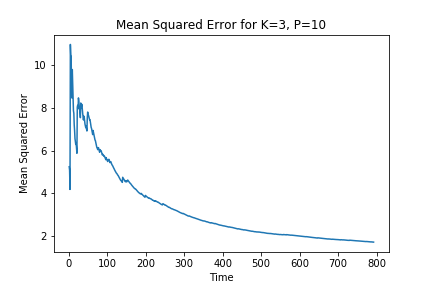
\includegraphics[width=\columnwidth]{TrainMSE}}
\caption{Training set mean squared error over time for K = 3 and 10 particles.}
\label{TrainMSE}
\end{center}
\vskip -0.2in
\end{figure}

We first examine mean squared error on the training set. As we see in Figure \ref{TrainMSE}, it decreases
over time as expected. The final MSE in this case is 1.721.

\begin{table}[ht]
\caption{Mean squared error statistics on the test set for various choices of K
(latent dimensionality) and P (number of particles)}
\label{sample-table}
\vskip 0.15in
\begin{center}
\begin{small}
\begin{sc}
\begin{tabular}{lcccc}
\toprule
(K, P) & Mean & Std Dev & Min & Max \\
\midrule
(2, 2)  & 2.924 & 0.355 & 2.512 & 3.585 \\
(2, 5)  & 2.981 & 0.387 & 2.552 & 3.711 \\
(3, 5)  & 2.540 & 0.182 & 2.408 & 2.900 \\
(3, 10) & 2.838 & 0.507 & 2.326 & 3.639 \\
(5, 2)  & 2.329 & 0.086 & 2.199 & 2.441 \\
(5, 10) & 2.367 & 0.088 & 2.251 & 2.519 \\
(5, 20) & 2.357 & 0.062 & 2.250 & 2.413 \\
\bottomrule
\end{tabular}
\end{sc}
\end{small}
\end{center}
\vskip -0.1in
\end{table}

\subsection{Cumulative Take Rate}

\subsection{Hyperparameter Cross Validation}

\subsection{User Preference Drift}

\section{Conclusion}

\nocite{kawale2015efficient}
\nocite{wang2017online}
\nocite{zhao2013interactive}
\nocite{cherkassky2013sequential}
\nocite{arulampalam2002tutorial}

\bibliographystyle{icml2018}
\bibliography{report}

\end{document}
